\subsection{扩展案例：三轮洪涝交通核查}
瓦伦西亚案例在同一对话中先筛查区域主干路，再将范围缩小到 Paiporta 和 Benetússer，最后应追问单独核查 Benetússer 的本地道路。每轮由 Pi 传入对应市镇和道路类别，调用空间分析和制图工具。工作台保存各轮地图、路段清单与分析编号。

\begin{table}[H]
\centering
\caption{道路核查三轮的范围、参数和结果。长度为分析支持域内的道路中心线；片段数不是道路条数。}
\label{tab:transport-turns}
\small
\begin{tabularx}{\linewidth}{@{}p{25mm}>{\raggedright\arraybackslash}X r r r@{}}
\toprule
任务 & 实际参数与分析范围 & 片段 & 淹没区（m） & 洪水痕迹（m）\\
\midrule
区域主干路 & 18 个相交候选市镇，17 个有联合资料覆盖；八类干线及连接道 &241&19.67&22\,436.27\\
两市镇主干路 & Paiporta 与 Benetússer；保持来源及类别不变 &23&0.00&2\,002.67\\
本地道路 & 仅 Benetússer；另起本地道路口径 &46&0.00&2\,091.04\\
\bottomrule
\end{tabularx}
\end{table}

\paragraph{第一轮：区域主干路筛查。}
表~\ref{tab:transport-turns} 第一轮纳入 141.66 km 道路中心线。10 个市镇有道路与洪涝证据重叠，累计 241 个片段。淹没区重叠 19.67 m，位于 Picanya 的 CV-36；另有约 22.44 km 与洪水痕迹重叠。约 372 m 带桥隧标记，供后续核对结构高程。空间分布见图~\ref{fig:transport-region}。

例如，Catarroja 的 V-31 有一段约 735.49 m 的洪水痕迹重叠，中心点为西经 $0.389512^\circ$、北纬 $39.396884^\circ$。地图编号对应路段清单中的位置，可据此查阅事件档案。

\paragraph{第二轮：缩小到两个市镇。}
两镇均基本处于联合资料覆盖范围内。Paiporta 所选路网长约 6.33 km，与洪水痕迹重叠约 2.00 km；其中 CV-400 为 1\,235.93 m，CV-407 为 699.50 m，位置见图~\ref{fig:transport-focus}。Benetússer 没有符合当轮筛选条件的历史道路，比例留空。

\paragraph{第三轮：改查 Benetússer 本地道路。}
调整道路类别后，Benetússer 纳入 18.62 km 本地道路，其中约 2.09 km 与洪水痕迹重叠，占 11.23\%，共 46 个片段。按道路名称汇总，Carrer del Moll de l'Estació 重叠 488.90 m；按单个片段排序，Carrer del Mont Alt 最长，为 376.41 m。成果可按道路汇总，也可按片段定位（图~\ref{fig:transport-local}）。

\clearpage
\begin{landscape}
\thispagestyle{empty}
\noindent\begin{minipage}[c][148mm][c]{\linewidth}
\centering
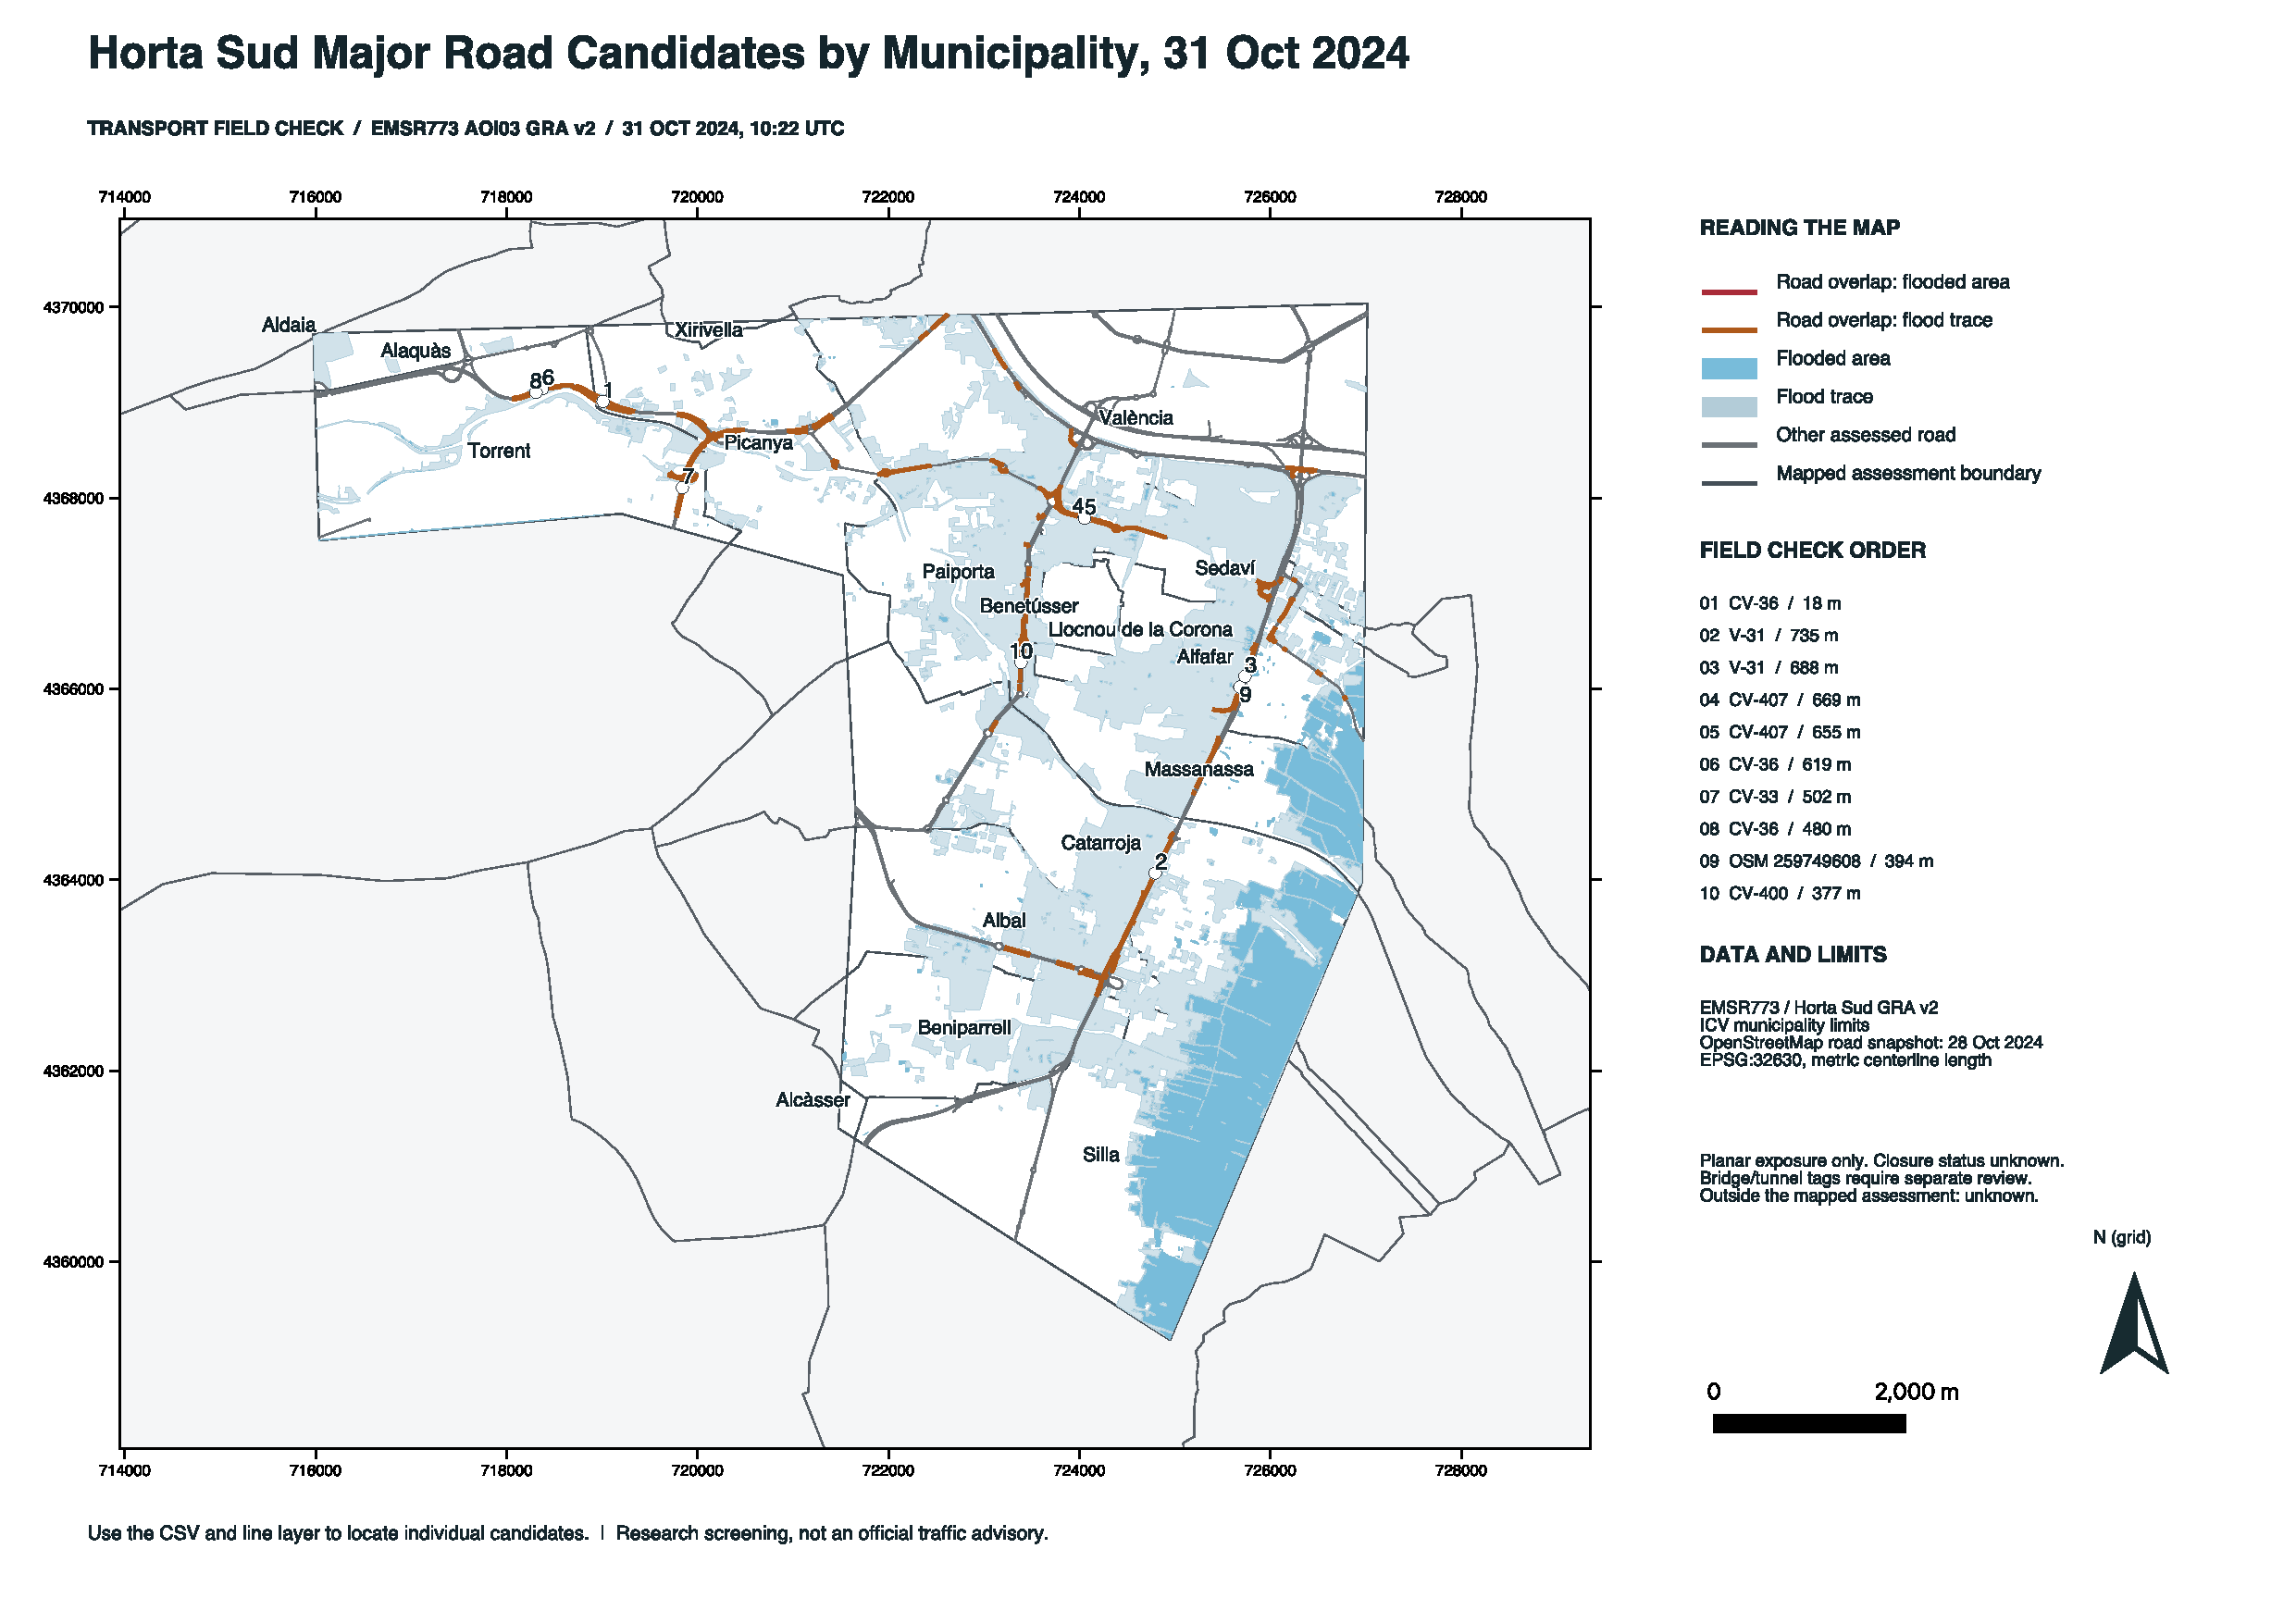
\includegraphics[width=\linewidth,height=136mm,keepaspectratio]{evidence/monitoring/transport/outputs/horta_sud_major_roads_by_town_01/transport.pdf}
\captionsetup{hypcap=false}
\captionof{figure}{Horta Sud 区域主干道路初筛。红色和棕色线段分别表示与观测淹没区和洪水痕迹重叠的道路片段；浅灰标示资料范围外及边界背景。}
\label{fig:transport-region}
\end{minipage}\par
\noindent\hfill{\sffamily\small\color{reportmuted}\thepage}\hfill\mbox{}
\end{landscape}

\begin{landscape}
\thispagestyle{empty}
\noindent\begin{minipage}[c][148mm][c]{\linewidth}
\centering
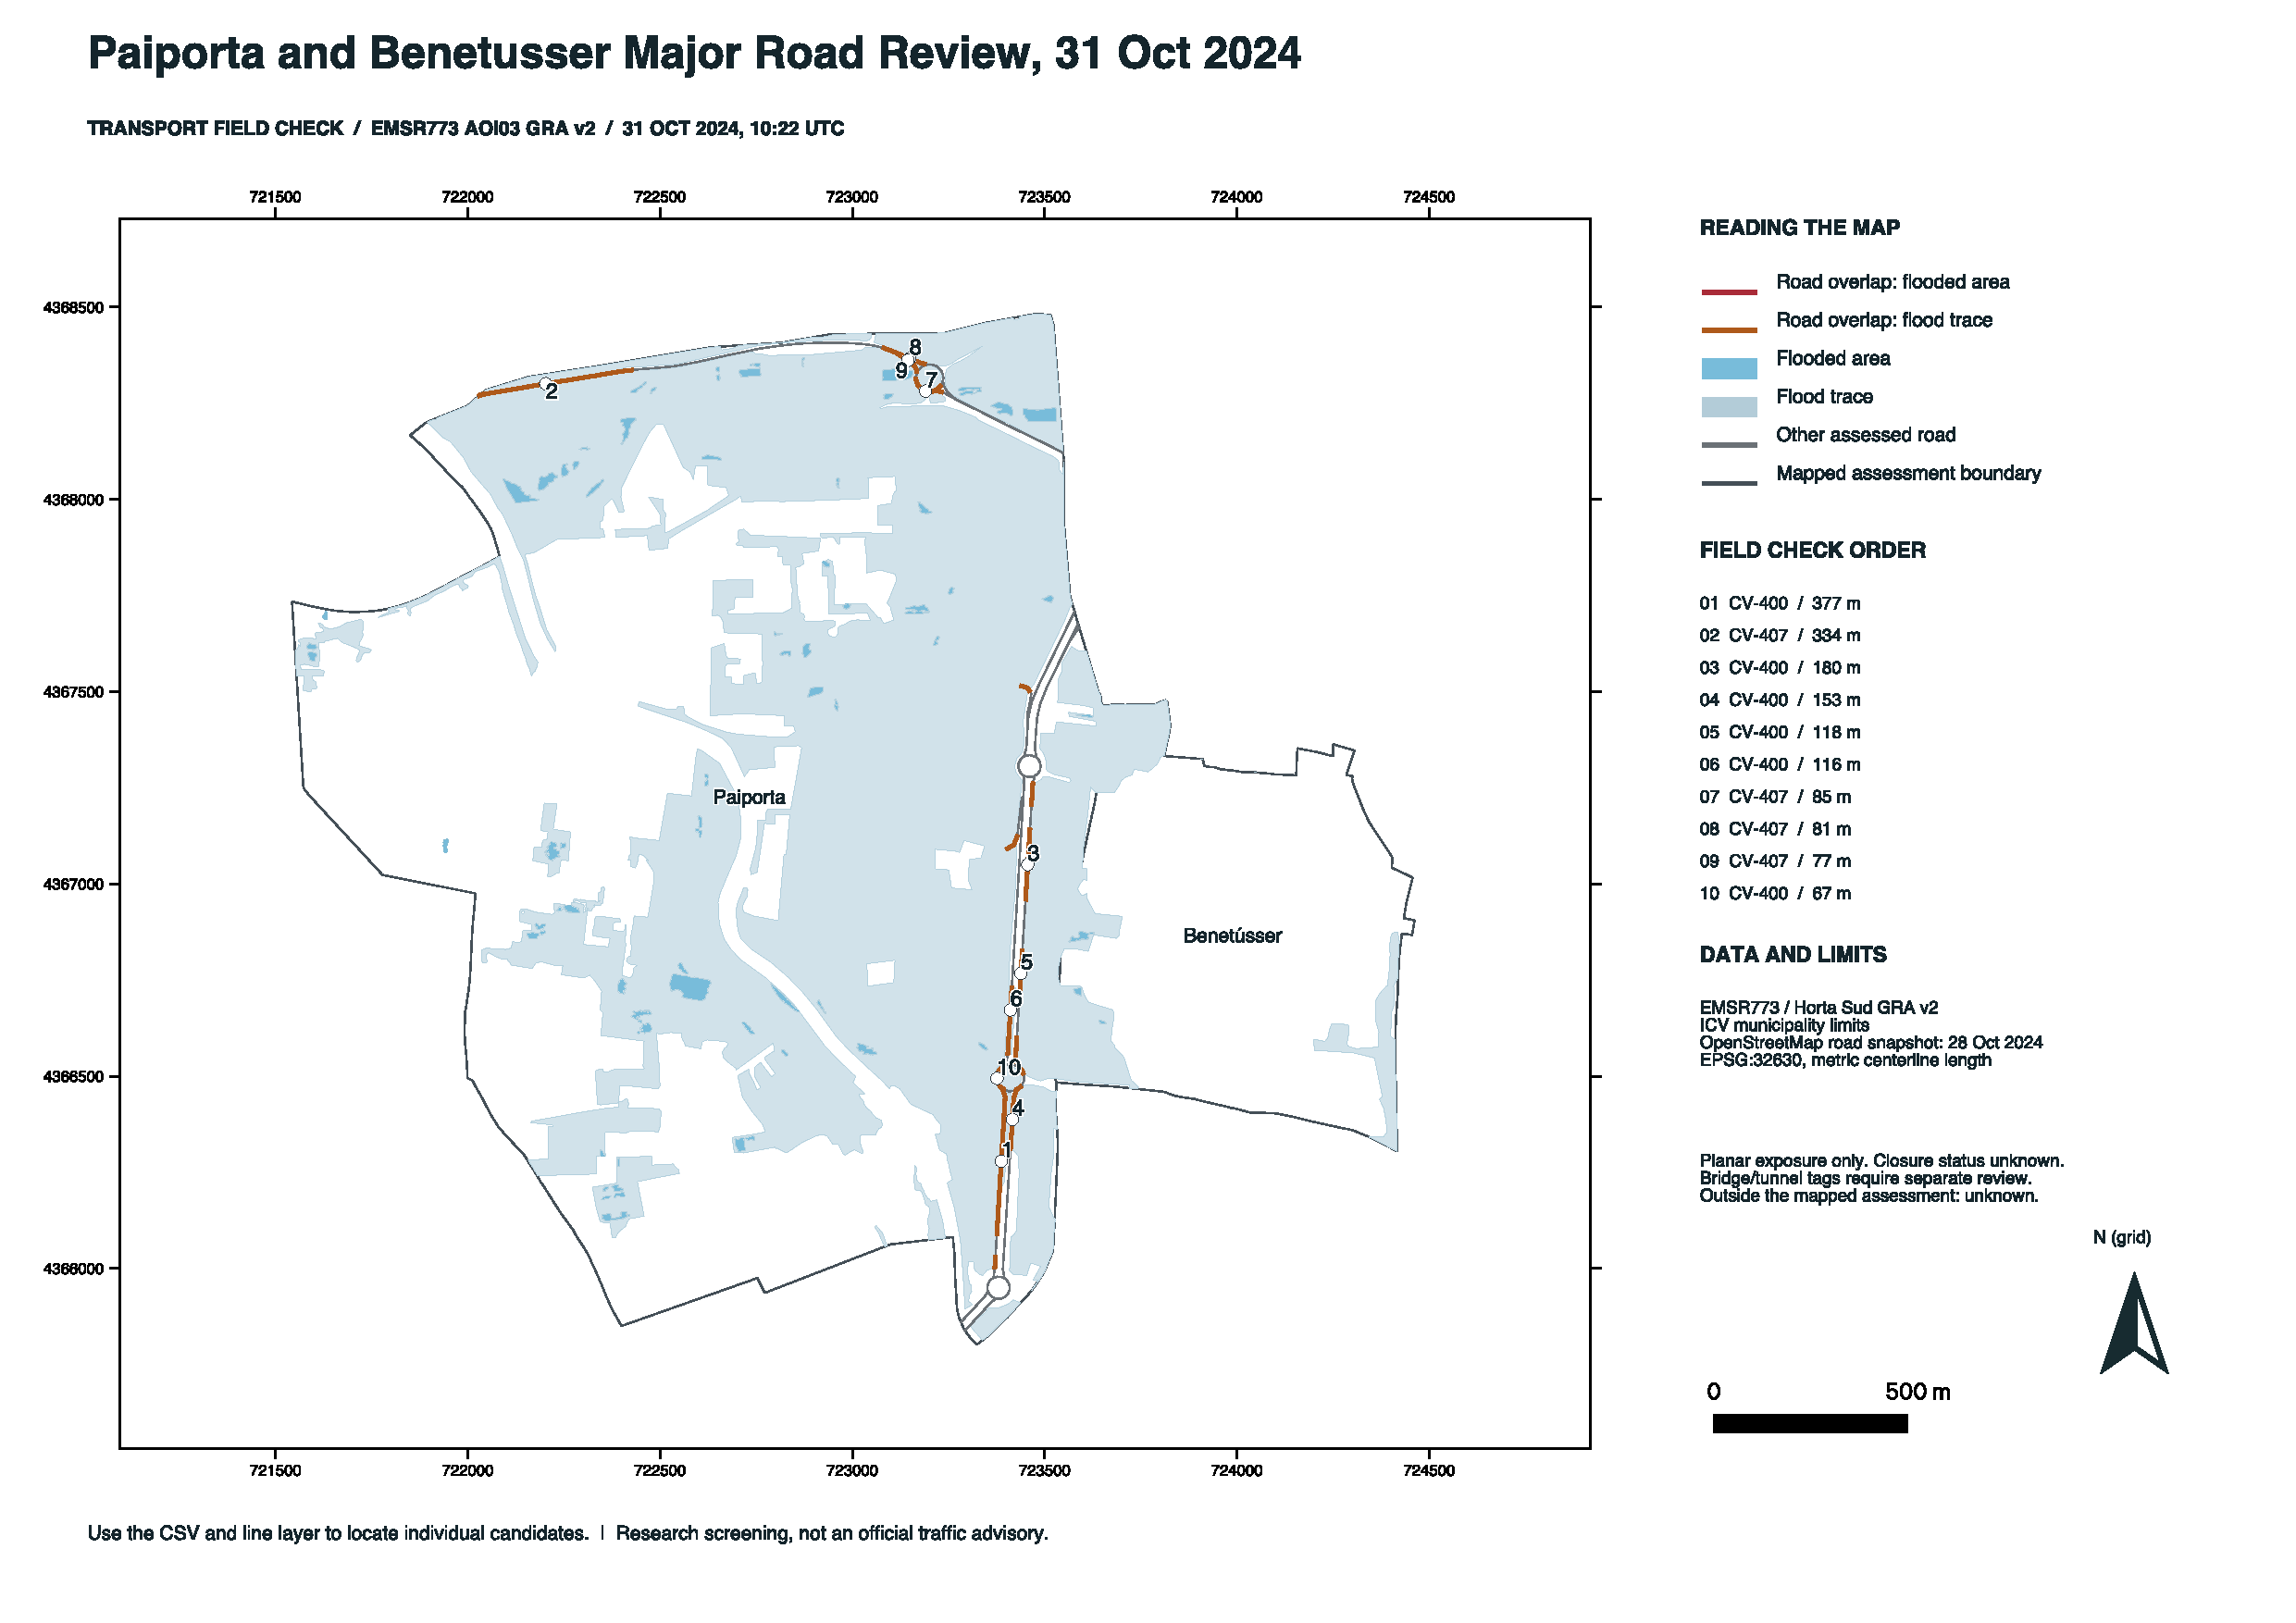
\includegraphics[width=\linewidth,height=136mm,keepaspectratio]{evidence/monitoring/transport/outputs/horta_sud_paiporta_benetusser_major_roads_02/transport.pdf}
\captionsetup{hypcap=false}
\captionof{figure}{Paiporta 与 Benetússer 主干道路核查。沿用区域初筛的资料和道路类别，编号为本轮候选片段的核查次序。}
\label{fig:transport-focus}
\end{minipage}\par
\noindent\hfill{\sffamily\small\color{reportmuted}\thepage}\hfill\mbox{}
\end{landscape}

\begin{landscape}
\thispagestyle{empty}
\noindent\begin{minipage}[c][148mm][c]{\linewidth}
\centering
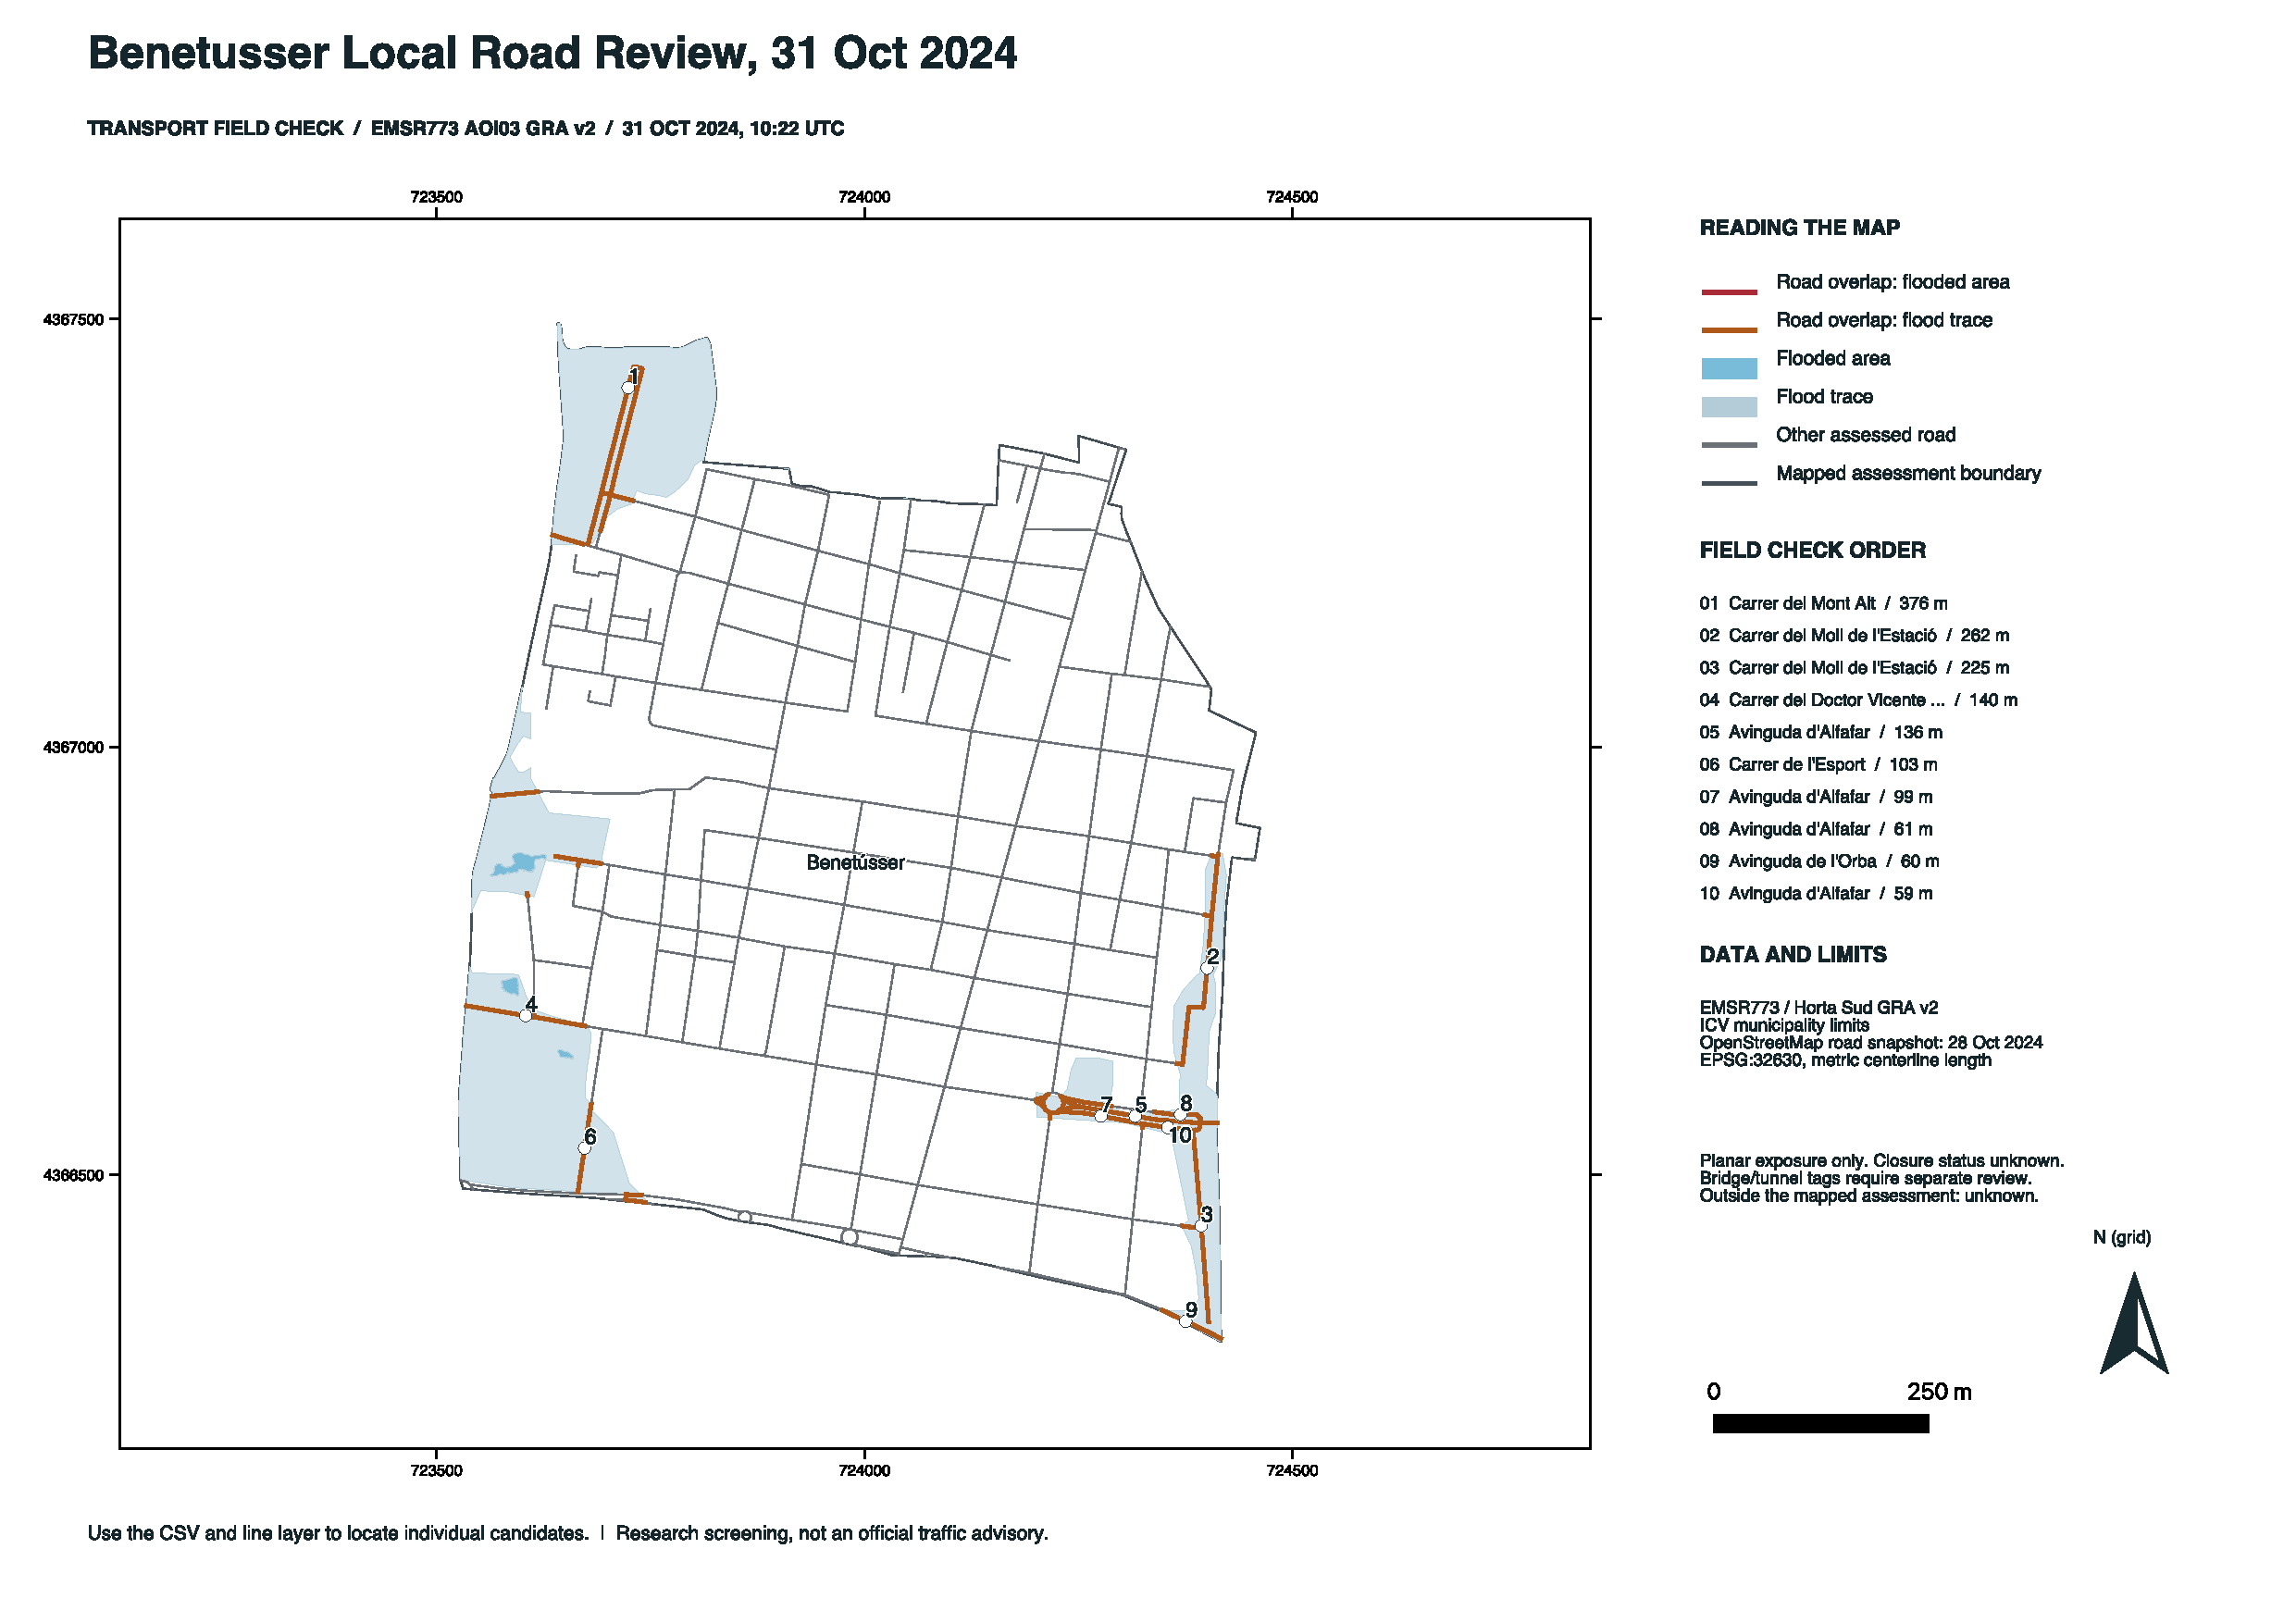
\includegraphics[width=\linewidth,height=136mm,keepaspectratio]{evidence/monitoring/transport/outputs/horta_sud_benetusser_local_roads_03/transport.pdf}
\captionsetup{hypcap=false}
\captionof{figure}{Benetússer 本地道路复核图。与前图相比，研究问题改为四类本地道路；棕色路段只表示与洪水痕迹重叠。}
\label{fig:transport-local}
\end{minipage}\par
\noindent\hfill{\sffamily\small\color{reportmuted}\thepage}\hfill\mbox{}
\end{landscape}
